\documentclass[11pt, a4paper]{article} % required for every LaTeX document
% specify fontsize and the paper, default is US letter

% everything after a % is a comment, unless it is escaped (\%)

% geometry is basically required for every LaTeX document – default LaTeX spacing looks really weird
\usepackage[bottom=2 cm, top=2 cm, left=2 cm, right=1.5 cm]{geometry}

% the ams packages contain a lot of commands necessary for setting mathematical formulae in LaTeX
% if your document contains more than trivial formulae, chances are you'll need them.
% if you are unsure, you can check requirded symbols at
% http://detexify.kirelabs.org/classify.html
\usepackage{amsmath, amsfonts, amssymb, amsthm}

% specify a nicer font than the default LaTeX font (Computer Modern)
% only works for modern tex interpreters like XeLaTeX and luaLaTeX
\usepackage{fontspec}
\setmainfont{Linux Biolinum}

% set the document language to German, if required
% polyglossia requires a modern interpreter, use babel if using pdflatex

%\usepackage{polyglossia}
%\setdefaultlanguage{german}
% or
%\usepackage[ngerman]{babel}


% Tikz is very useful for setting graphics directly in LaTeX, but fairly complex
% apart from stackoverflow, the documentation and the texample page are quite helpful
% They can be found at
% https://pgf-tikz.github.io/pgf/pgfmanual.pdf
% https://texample.net/tikz/examples/
\usepackage{tikz}

% package to add hyperlinks directly to the PDF
\usepackage[colorlinks=true, breaklinks=true]{hyperref}

% some other cool packages to check out:
%\usepackage{siunitx} % for properly setting dimensional qualities with units
%\usepackage{parskip} % for elegant paragraph handling
%\usepackage{fancyhdr} % for fancy headers/footers!
%\usepackage{comment} % for block comments. Useful for larger documents
%\usepackage{algoritm2e} % for elegant pseudocode
%\usepackage{listings} % for elegant setting of code
%\usepackage{caption} % for advanced float captioning

% https://www.overleaf.com/learn

% LaTeX allows users to define their own commands
% this feature is particularly useful to shorten commonly-used, long expressions, e.g. the expectation value and Variance:
\newcommand{\ev}{\mathbb{E}}
\newcommand{\var}{\mathrm{Var}}


% set the document header
\title{GumbelTalks \LaTeX\ Intro\\
\large An example exercise sheet using \LaTeX}
\author{Leon Rauschning}
\date{15/4/23} % date of the compilation, if not specified


\begin{document}
\maketitle % this automagically generates a header for the document
% how the header looks exactly can be modified by the documentclass and LaTeX code in the header
\section{Solve a linear equation}
In exercise 1, we will demonstrate how to solve a linear equation.\\ %\\ is a line break
The given equation is of form
\begin{equation} % \begin opens an environment (in this case, the equation environment)
	y = mx + t % the equation environment is already in math mode; we do not need to enter it separately
	\label{eqn-lineq} % label the equation, to refer to the number later
\end{equation}
, with $m$ being the \emph{slope} and $t$ the \emph{intercept}.
We solve for $x$:
\begin{eqnarray*} % these equations are not important, disable numbering with *
	y =& mx + t\\ % & is an alignment character; in this case, it tells LaTeX
	y - t =& mx\\ % to align these equations on the = sign
	x =& \frac{y-t}{m}
\end{eqnarray*}
With $y=6$, $t=2$ and $m=2$ given in the exercise, we can show that
$$x=2$$ % this is display math mode
holds.
The same result could also be obtained using \texttt{scipy.linalg.solve} \textbf{or any other equation solving software}. % \texttt sets the text in a mono ("TeleType") font, \textbf in a bold font
\qed

% two empty lines denote a new paragraph in LaTeX
See also Fig.~\ref{fig-lineq} for a graphical illustration of the solution of Eqn.~\ref{eqn-lineq}. % ~ is a non-breaking space. It tells LaTeX not to put a linebreak where it doesn't belong.
% this is commonly used in references and names/titles

\begin{figure}[ht]
	% figure is also an environment, but it's a bit special as it is a float.
	% that means that the text may not be at the same location in the PDF as it is in the TeX source code.
	% the [ht] is a float placement specifier telling LaTeX to place the table right here, if possible [h – here], or failing that, on the top of the next page [t – top]
	% note that LaTeX will always preserve the order of floats, so placing a float with [h] or [h!] may cause other figures to be placed right before that float, which can look pretty bad.
	\centering
	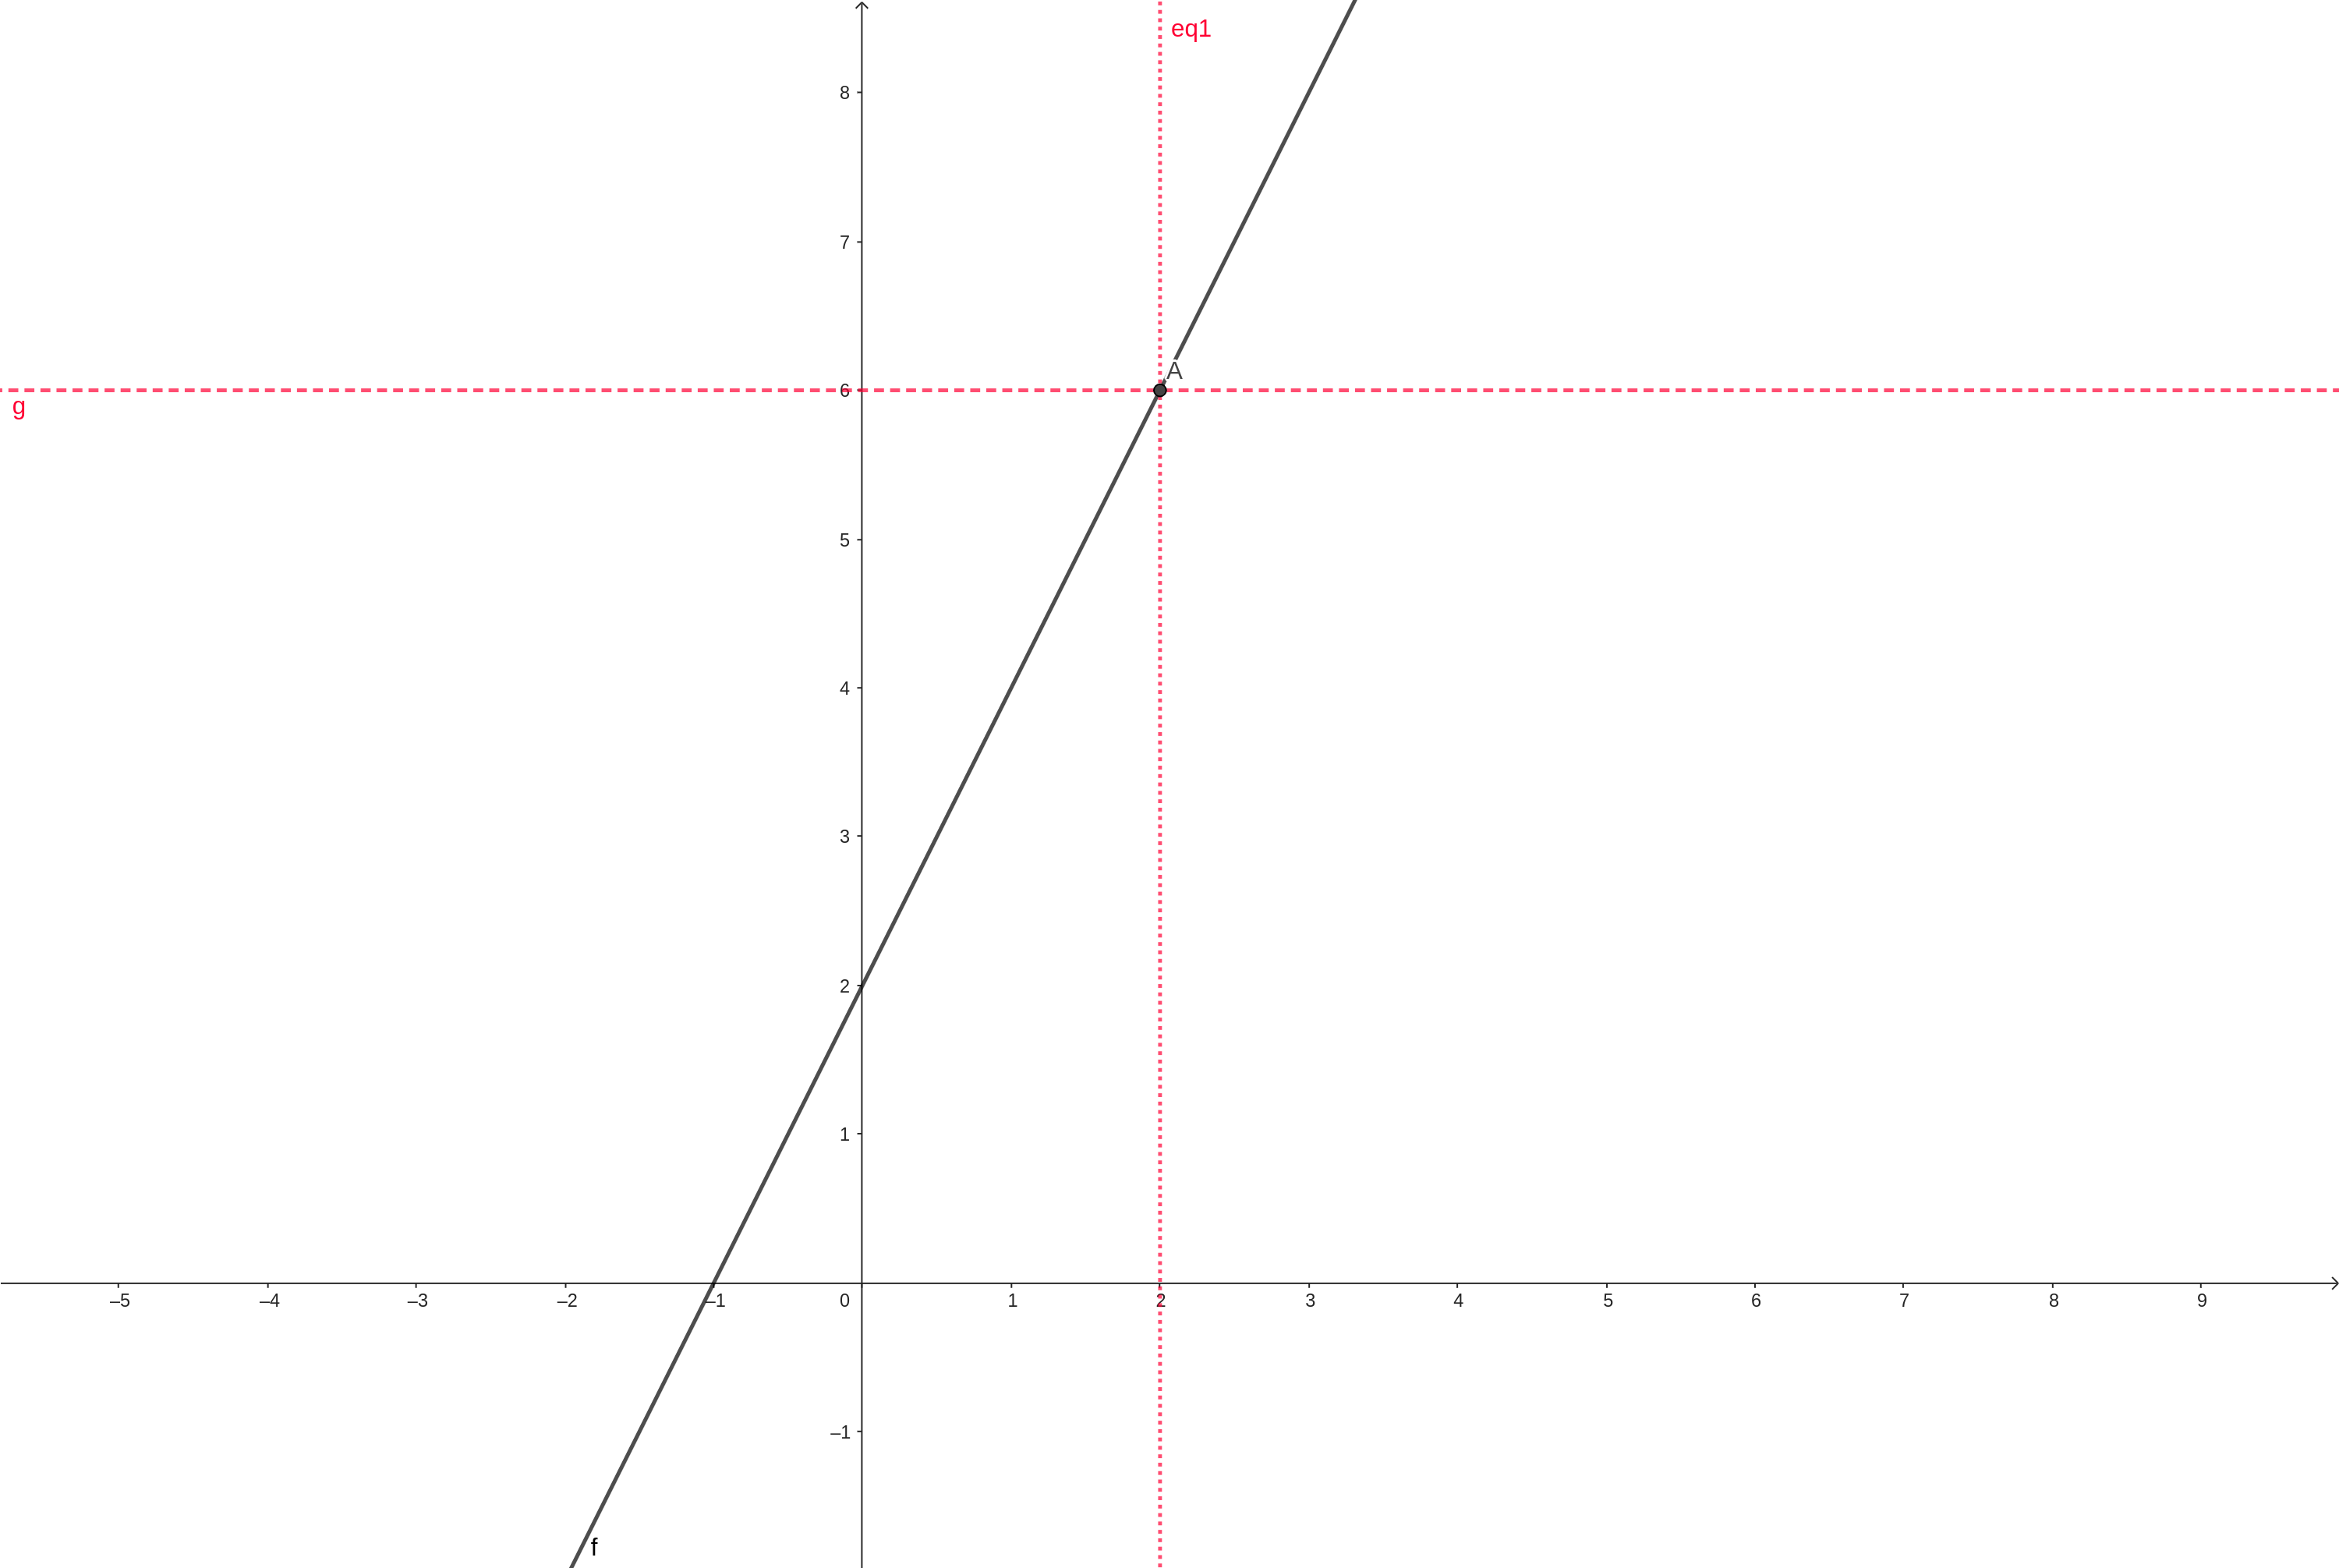
\includegraphics[width=.7\textwidth]{fig1-lineq.png}
	% \textwidth is predefined by latex as the width available for text setting – this is very useful when sizing images
	\label{fig-lineq}
	\caption{Graphical solution to Eqn.~\ref{eqn-lineq} using GeoGebra}
\end{figure}

\section{Everyone loves pie!}
In exercise 2, we will demonstrate an approximation for $\pi$. % greek letters can be specified as unicode characters in modern latex distributions (see below for an example).
% but it is frequently more convenient to use the predefined commands for them
We introduce the Leibniz series $\mathcal{L}$:
$$ % a long expression can be spread over multiple lines
\mathcal{L} = % mathcal gives us fancy letters that are suitable for names
1 - \frac{1}{3} + \frac{1}{5} - \frac{1}{7} + \frac{1}{9} \ldots % a single command can take multiple arguments, as is the case for \frac!
= \sum_{n=0}^\infty \frac{(-1)^n}{2n + 1}% _ is a subscript, ^ is a superscript. If only one letter/command is used as a sub/superscript, the brackets can be left out
$$

This series can be shown to converge to $\frac{\pi}{4}$ by forming it into a geometric series:
\begin{eqnarray*}
	\mathcal{L} =& \sum_{n=1}^\infty \frac{(-1)^n}{2n+1}\\
	=& \sum_{n=0}^\infty (-1)^n \int_0^1 x^{2k} \,\mathrm{d}x\\ % \, sets a small space, \. a big space; \mathrm switches to roman (»normal«) font. This way the integral looks nice
	% if using an integral more often, it is convenient to define a command for this (see below)
	=& \int_0^1 \sum_{n=0}^\infty (-x^2)^n\,\mathrm{d}x
\end{eqnarray*}
% we will need the integral a bit more from here on, so define a command for it:
\newcommand{\idx}{\,\mathrm{d}x}

Applying the formula for geometric series to the term inside the integral, we are able to eliminate the infinite series from this expression:
$$\sum_{n=0}^\infty(-x^2)^n = \frac{1}{1-(-x^2)} = \frac{1}{x^2 + 1}$$
Ultimately leaving us with a simple integral:
$$\mathcal{L} = \int_0^1 \frac{1}{x^2 + 1} \idx
= [\arctan(x)]^1_0 % many common functions have predefined commands
= \arctan(1)
= \frac{\pi}{4}
$$

Thus, we have shown that the Leibniz series can be used as a simple way to compute an approximation of $\pi$.
An example for the approximation of $\pi$ in this manner is given in Table~\ref{tab-pi}.
\qed


\begin{table}[hb] 
	\caption{This table shows the approximation of $\pi$ by the Leibniz sum as more terms are added to the sum.
	Correct digits are written in bold.
	The values were calculated using python: \texttt{print(4*sum(map(lambda x: ((-1)**x)/((2*x)+1), range(n))))}
	}
	\label{tab-pi}
	\centering % to have the table centre-aligned
	\begin{tabular}{l | c } % the tabular environment contains the actual table.
		% the {l | c} tells LaTeX how the table should be formatted.
		% in this case, the table has one left-aligned column, a vertical line and one centre-aligned columns
		Number of terms ($n$) & Value\\ % the cells in a row are separated by alignment (&) characters
		\hline % draw a line below the names
		1 & 4\\
		10 & \textbf{3}.0418396\\
		100 & \textbf{3.1}315925\\
		1000 & \textbf{3.14}05926\\
		10,000 & \textbf{3.141}4929\\
		100,000 & \textbf{3.1415}826\\
		1,000,000 & \textbf{3.14159}16\\
		
	\end{tabular}
\end{table}
\end{document}
